\documentclass[a4paper,11pt,titlepage,openany]{jsbook}
\usepackage[utf8]{inputenc}

% -- 設定ファイルの読み込み -- %
\usepackage[dvipdfmx]{graphicx}
\usepackage{wrapfig}
\usepackage{amsmath}
\usepackage{geometry}
\usepackage{comment}
\usepackage{bm}
\usepackage{fancyvrb}

\usepackage[dvipdfmx]{hyperref}
% for hyperref
\usepackage{pxjahyper}
\hypersetup{% hyperrefオプションリスト
setpagesize=false,
 bookmarksnumbered=true,%
 bookmarksopen=true,%
 colorlinks=true,%
 linkcolor=blue,
 citecolor=blue,
}

% ページの余白を1.25インチにする
\geometry{
	left=1.25truein,
	right=1.25truein,
	top=1.25truein,
	bottom=1.25truein,
}

%ページの上下に出力される図と図の間のスペース
\setlength\floatsep{5.0pt} %dblfloatsep

%ページの上下に出力される図と本文の間のスペース
\setlength\textfloatsep{5.0pt} %dbltextfloatsep

%ページの途中に出力される図と本文の間のスペース
\setlength\intextsep{5.0pt}

%図の参照
\newcommand{\Fig}[1]{Fig.\ref{fig:#1}}
%表の参照
\newcommand{\Tb}[1]{Tab.\ref{tab:#1}}
%式の参照
\newcommand{\Eq}[1]{Eq.(\ref{eq:#1})}

\renewcommand{\figurename}{Figure}
\renewcommand{\tablename}{Table}

\makeatletter
 \renewcommand{\theequation}{%
   \thechapter.\arabic{equation}}
  \@addtoreset{equation}{chapter}
  
  \renewcommand{\thefigure}{
  \thechapter.\arabic{figure}}
  \@addtoreset{figure}{chapter}
  
  \renewcommand{\thetable}{
    \thechapter.\arabic{table}}
  \@addtoreset{table}{chapter}
\makeatother

%%%%%%%%%%%%%%%%%%%%%%%%%%%%%%%%%%%%%%%%%%%%%%%%%%%%%%%%%%
\begin{document}
%%% !---- 表紙 ----! %%%
\begin{titlepage}
	\begin{center}
		\vspace{25truemm}
		{\huge \bf{特別研究報告}\par}
		\vspace{10truemm}
		{\huge \underline{題目}\par}
		\vspace{5truemm}
		{\huge 二列配列イオンの余剰マイクロ運動抑制を\\目指した電場評価方法の開発\par}
		\vspace{15truemm}
		{\huge \underline{指導教員}\par}
		\vspace{5truemm}
		{\huge 田中 \ 歌子 \ 講師\par}
		\vspace{15truemm}
		{\huge \underline{報告者}\par}
		\vspace{5truemm}
		{\huge 西本 \ 涼介\par}
		\vspace{15truemm}
		{\huge 2022年2月9日\par}
		\vspace{15truemm}
		{\huge 大阪大学 \ 基礎工学部 \ 電子物理科学科 \\ エレクトロニクスコース}
	\end{center}
\end{titlepage} %表紙の裏として一ページの余白が入る

%%% !---- 前付 ----! %%%
\frontmatter
	% -- 概論 -- %
	\chapter{概要}
卒業論文
	% -- 目次 -- %
	\setcounter{tocdepth}{2}
	\tableofcontents

%%% !---- 本文開始 ----! %%%
\mainmatter %奇数ページから開始される
	% -- 序論 -- %
	\chapter{序論}
冷却原子の運動状態と内部状態をレーザーで制御することで量子コンピュータや量子シミュレーションが実現できることが提案されて久しい\cite{Cirac_1995}.冷却原子を準備する装置の一つに静電場と高周波電場による電磁場を利用してイオンを空間中に閉じ込めるPaulトラップと呼ばれる装置が挙げられる.Paulトラップは量子情報処理の実験の多くに使用されている.現在,一列に並ぶイオンを用いた79-qubitの安定な制御が可能となっている\cite{Wright_2019}.また,イオンの配列を一列から二次元へと拡張することで量子コンピュータや量子シミュレーションの応用範囲が広がることが指摘されており\cite{Cirac_2000},二次元配列として捕獲されたイオンを用いてフラストレーション効果を調査した報告などがある\cite{Mielenz_2016}.

電極の非対称性などに起因してトラップ内に発現する浮遊電場の存在はイオンに余剰マイクロ運動と呼ばれる微小振動を引き起こす.安定な量子系を確立するにあたり,余剰マイクロ運動がよく補正されていることは前提条件として要求される.現在,一列配列イオンの余剰マイクロ運動の補正方法は多数報告されているが\cite{Berkeland_1998}\cite{Chen_2020}\cite{Timm_2015},二次元配列のイオンの余剰マイクロ運動の補正手法は確立されていない.

イオンは電場の影響を敏感に受ける.そのため,単一イオンをセンサーとしてトラップ内の浮遊電場の解析\cite{Narayanan_2011}や電極表面に存在する電気ノイズの解析\cite{Danii_2014}が行われている.様々な構造を持つ電極によってイオンの制御が試みられている中,各トラップに存在するノイズの検出は非常に重要となっている.

当研究グループでは,微細加工技術を施したプレーナートラップを用いてイオンを二列に捕獲することを可能としており\cite{Tanaka_2021},二列配列イオンにおける電場の検出を試みている.よく制御された二列配列イオンが確立されれば,量子コンピュータや量子シミュレーションの大規模化に加え,イオン列間に生じる電位障壁に対するトンネル効果の実証実験や,巨視的現象である摩擦の原子レベルでの検証実験などへの応用が期待される\cite{Tanaka_2021}\cite{L-Timm_2021}.
	% -- 理論 -- %
	\section{理論}
\subsection{イオントラップ}
電荷を持つイオンは電場によって力を受けることから,電磁場を用いることで空間に閉じ込めることが可能になっている.これを可能にする装置をイオントラップと呼ぶ.電磁気学において,アーンショーの定理と呼ばれる定理が知られており,この定理によれば静電ポテンシャルを記述するラプラス方程式の解に極大値および極小値が表れない.つまり,静電場のみを用いてイオンを捕獲することが不可能になっている.イオンを閉じ込めるためには,静電場と静磁場を使ったペニンブトラップ,あるいはrf(radio frequency)電場と静電場を用いたパウルトラップが主に使用される.本研究では後者のパウルトラップの原理を応用させた平面型のイオントラップ.プレーナートラップを使用してイオンの捕獲を行っていることから,パウルトラップについて述べる.
\subsection{パウルトラップ}
\subsubsection{rf擬ポテンシャル}
\large
\begin{align}
	\Phi_{\rm eff}(x,y,z) = \frac{e}{4m\Omega_{\rm rf}}|\vec{E}(x,y,z)|^2
\end{align}
\normalsize


\subsubsection{イオンの運動}
Mathieu方程式
\large
\begin{align}
	\frac{{\rm d^2}r_i}{{\rm d}t^2} + [a_\alpha + 2q_\alpha \cos (\Omega_{\rm rf} t)]\frac{\Omega_{\rm rf}^2}{4}r_i = 0. \quad (i = x,y,z)
\end{align}
\normalsize
\subsubsection{余剰マイクロ運動}
浮遊電場が存在する場合のMathieu方程式
\large
\begin{align}
	\frac{{\rm d^2}r_i}{{\rm d}t^2} + [a_i + 2q_i \cos (\Omega_{\rm rf} t)]\frac{\Omega_{\rm rf}^2}{4}r_i = \frac{e\vec{E}_{\rm stray}\cdot \hat{r}_i}{m}. \quad (i = x,y,z)
\end{align}
\normalsize
rfに起因,レーザーによって冷却することができない
\clearpage
\subsection{プレーナートラップ}
\begin{figure}[h]
	\begin{center}
		\begin{minipage}{0.48\linewidth}
			\begin{center}
			\includegraphics[width = 0.98\columnwidth]{./theory/figure/PaulTrap_3Dto2D_3DTrap.png}
			\end{center}
		\end{minipage}
		\begin{minipage}{0.48\linewidth}
			\begin{center}
			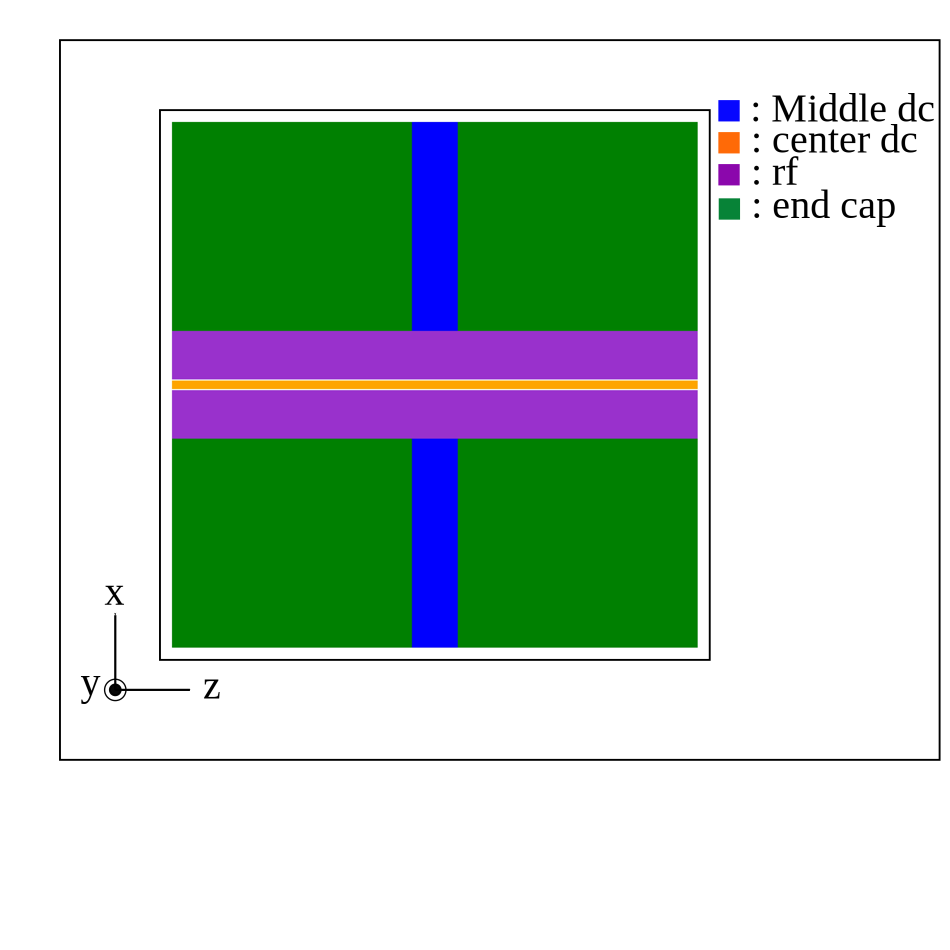
\includegraphics[width = 0.98\columnwidth]{./theory/figure/PaulTrap_3Dto2D_2DTrap.png}
			\end{center}
		\end{minipage}
	\end{center}
\end{figure}
\subsubsection{電極の仕様}
\begin{figure}[h]
	\begin{center}
		\includegraphics[width = 0.5\linewidth]{./theory/figure/named_electrode.png}
		\caption{本実験で使用するプレーナートラップの電極モデル}
		\label{fig:Named_PlannerTrap}
	\end{center}
\end{figure}
\subsubsection{矩形電極が作る静電ポテンシャル}
\begin{figure}[h]
	\begin{center}
		\includegraphics[width = 0.5\linewidth]{./theory/figure/Potential_of_rect-electrode.png}
		\caption{$(z_1,x_1),(z_2,x_2)$で指定される矩形が任意の点$(x,y,z)$に形成する静電ポテンシャル}
		\label{fig:Potential_from_rect-electrode}
	\end{center}
\end{figure}
\begin{align}\label{eq:rectangle_electrode}
	\phi(x,y,z) = \frac{V}{2\pi} \left\lbrace \arctan \left[ \frac{(x_2 - x)(z_2 - z)}{y\sqrt{y^2 + (x_2 - x)^2 + (z_2 - z)^2}}\right] - \arctan \left[ \frac{(x_1 - x)(z_2 - z)}{y\sqrt{y^2 + (x_1 - x)^2 + (z_2 - z)^2}} \right]  \right.  \notag \\ 
	\left. -\arctan \left[ \frac{(x_2 - x)(z_1 - z)}{y\sqrt{y^2 + (x_2 - x)^2 + (z_1 - z)^2}}\right] + \arctan \left[ \frac{(x_1 - x)(z_1 - z)}{y\sqrt{y^2 + (x_1 - x)^2 + (z_1 - z)^2}} \right]  \right\rbrace 
\end{align}
\subsection{Mathematicaによるシミュレーション}
\subsubsection{DCポテンシャル}
\Eq{rectangle_electrode}より,dc電圧を計算するためには電極モデルを矩形の形に分割する必要がある.Mathematica上における電極の分割の様子を\Fig{rect_electrode}に示す.
\begin{figure}[h]
	\begin{center}
		\includegraphics[width = 0.4\linewidth]{./theory/figure/named_rect_electrode.png}
	\end{center}
	\caption{a}
	\label{fig:rect_electrode}
\end{figure}
各dc電極によってプレーナートラップ上の点$(x,y,z)$に形成される静電ポテンシャル$\Phi_{\rm DC}(x,y,z)$は,分割した各矩形が$(x,y,z)$に形成する静電ポテンシャルの重ね合わせで
\large
\begin{align}
	\Phi_{\rm DC}(x,y,z) = \phi_{\rm End1} + \phi_{\rm End2} + \phi_{\rm End3} &+ \phi_{\rm End4} + \phi_{\rm Mid1} + \phi_{\rm Mid2} \notag \\
	&+ \phi_{\rm Side1} + \phi_{\rm Side2} + \phi_{\rm center},
\end{align}
\normalsize
と表すことができる.
\begin{figure}[h]
			\begin{center}
				\includegraphics[width = 0.7\linewidth]{./theory/figure/PlannarTrap_3D_z=0.png}
			\end{center}
\end{figure}
\begin{figure}[h]
	\begin{center}
		\begin{minipage}{0.45\linewidth}
			\begin{center}
				\includegraphics[width = 1.2\columnwidth]{./theory/figure/dc_potential_example.png}
			\end{center}
		\end{minipage}
		\begin{minipage}{0.45\linewidth}
			\begin{center}
			\begin{tabular}{c|c} \hline \hline
				電極 & 印加電圧 ()V) \\ \hline
				End1 & 1.41 \\ \hline
				End2 & 1.41 \\ \hline
				End3 & 1.41 \\ \hline
				End4 & 1.41 \\ \hline
				Mid1 & -1.532 \\ \hline
				Mid2 & -1.532 \\ \hline
				Side1 & 0.222 \\ \hline
				Side2 & 0.222 \\ \hline
				center & 0.225 \\ \hline
			\end{tabular}
			\end{center}
		\end{minipage}
	\end{center}
\end{figure}
\subsubsection{Single-wellにおけるrf擬ポテンシャル}
\subsubsection{Double-wellにおけるrf擬ポテンシャル}
\subsection{レーザー冷却}
\subsection{画像処理によるイオン捕獲位置と電場の算出}
Pythonで,OpenCVとNumpyを使って画像処理を行うことでイオンの位置と,イオンの位置における電場の算出を行う.
\subsubsection{グレースケール化,二値化}
\subsubsection{イオンの検出および,捕獲位置と電場の算出方法}
	% -- 実験装置 -- %
	\chapter{実験装置}
\section{プレーナートラップ}
本実験で使用する電極の写真を\Fig{Using_PlannerTrap}に示す.
\begin{figure}[h]
	\begin{center}
		\includegraphics[width = 0.6\linewidth]{./experimental_setup/figure/Using_PlannerTrap.png}
		\caption{本実験で使用するプレーナートラップ}
		\label{fig:Using_PlannerTrap}
	\end{center}
\end{figure}

\section{光学系}
\Fig{optical_system}にイオン捕獲のためのレーザーの光学系を示す.
\begin{figure}[h]
	\centering
		\includegraphics[width = 0.7\linewidth]{./experimental_setup/figure/Optical_System.png}
		\caption{プレーナートラップに照射するレーザーの光学系}
		\label{fig:optical_system}
\end{figure}

\section{レーザー}
\begin{table}[h]
	\centering
		\caption{$^{40}{\rm Ca}^+$を捕獲するときに使用するレーザーの波長}
		\label{tb:use_laser}
			\begin{tabular}{c|c} \hline \hline
				基準周波数 & 632 nm \\ 
				$^{40}{\rm Ca}$のイオン化 & 423 nm, 375 nm \\
				$^{40}{\rm Ca}^+$の冷却 & 397 nm \\
				$^{40}{\rm Ca}^+$のリポンプ & 866 nm \\ \hline 
			\end{tabular}
\end{table}
イオントラップに使用するレーザーのビーム径とその強度をスリット走査型光ビームプロファイラ(THORLABS,BP209-VIS/M)とデジタルパワー\&エネルギーメータ(THORLABS,PM100D)およびフォトダイオードパワーセンサー(THORLABS,S120C)を用いて計測を行った.
まず,各レーザーの強度を\Tb{AllLaserPower}に示す.

\begin{table}[h]
	\begin{center}
		\caption{各レーザーのパワー一覧表}
		\label{tab:AllLaserPower}
		\begin{tabular}{c|c} \hline \hline
			波長 (nm) & 強度 ($\mu$W) \\ \hline
			375 &4.1 \\ \hline
			397 &17.4 \\ \hline
			423 &28.4 \\ \hline
			866 &700 \\ \hline
		\end{tabular}
	\end{center}
\end{table}

次に,ビーム径の計測結果を\Fig{AllLaserBeamProfile}に示す.

\begin{figure}[h]
	\begin{center}
	\begin{minipage}{0.48\linewidth}
		\includegraphics[width = 0.98\columnwidth]{./experimental_setup/figure/AllLaserXpos.jpg}
	\end{minipage}
	\begin{minipage}{0.48\linewidth}
		\begin{center}
		\includegraphics[width = 0.98\columnwidth]{./experimental_setup/figure/AllLaserYpos.jpg}
		\end{center}
	\end{minipage}
	\caption{4種類のレーザーのx,y方向についてのビームプロファイル結果}
	\label{fig:AllLaserBeamProfile}
	\end{center}
\end{figure}

そして,得られたビームプロファイルにガウシアンによるフィッティングを行った様子を\Fig{GaussianFitting}に示し,その結果を\Tb{GaussianFitting}にまとめている.\\

\begin{table}[h]
	\begin{center}
		\caption{ビームプロファイラで得られた各ビームのプロファイルにガウシアンフィッティングをかけて得られたパラメータ}
		\label{tab:GaussianFitting}
		\begin{tabular}{c|cc|cc} \hline \hline
			波長 (nm)&位置(x) ($\mu$m)&ビーム径(x) ($\mu$m) &位置(y) ($\mu$m)& ビーム径(y) ($\mu$m)\\ \hline
			375&-2600.82$\pm$0.035&6.96$\pm$0.049&-1051.14$\pm$0.028&9.37$\pm$0.04 \\
			397&-2606.08$\pm$0.026&24.21$\pm$0.037&-1056.17$\pm$0.016&18.45$\pm$0.023 \\
			423&-2611.55$\pm$0.05&30.20$\pm$0.072&1042.25$\pm$0.03&39.85$\pm$0.054 \\
			866&-2606.08$\pm$0.138&77.20$\pm$0.196&-1054.24$\pm$0.06&54.72$\pm$0.085 \\\hline
		\end{tabular}
	\end{center}
\end{table}

\clearpage

\begin{figure}[h]
	\begin{center}
	%%%12
	\begin{minipage}{0.48\linewidth}
	\begin{center}
			\includegraphics[width = 0.98\columnwidth]{./experimental_setup/figure/375GaussianFittingXpos.jpg}
	\end{center}
	\end{minipage}
	\begin{minipage}{0.48\linewidth}
	\begin{center}
			\includegraphics[width=0.98\columnwidth]{./experimental_setup/figure/375GaussianFittingYpos.jpg}
	\end{center}
	\end{minipage}
	%%%34
	\begin{minipage}{0.48\linewidth}
	\begin{center}
		\includegraphics[width = 0.98\columnwidth]{./experimental_setup/figure/397GaussianFittingXpos.jpg}
	\end{center}
	\end{minipage}
	\begin{minipage}{0.48\linewidth}
	\begin{center}
		\includegraphics[width=0.98\columnwidth]{./experimental_setup/figure/397GaussianFittingYpos.jpg}
	\end{center}
	\end{minipage}
	%%%56
	\begin{minipage}{0.48\linewidth}
	\begin{center}
		\includegraphics[width = 0.98\columnwidth]{./experimental_setup/figure/423GaussianFittingXpos.jpg}
	\end{center}
	\end{minipage}
	\begin{minipage}{0.48\linewidth}
	\begin{center}
		\includegraphics[width=0.98\columnwidth]{./experimental_setup/figure/423GaussianFittingYpos.jpg}
	\end{center}
	\end{minipage}
	%%%78
	\begin{minipage}{0.48\linewidth}
	\begin{center}
		\includegraphics[width = 0.98\columnwidth]{./experimental_setup/figure/866GaussianFittingXpos.jpg}
	\end{center}
	\end{minipage}
	\begin{minipage}{0.48\linewidth}
	\begin{center}
		\includegraphics[width = 0.98\columnwidth]{./experimental_setup/figure/866GaussianFittingYpos.jpg}
	\end{center}
	\end{minipage}
	\caption{各波長に対してx,y方向それぞれのビームプロファイルにガウシアンフィッティングをかけた結果}
	\label{fig:GaussianFitting}
	\end{center}
\end{figure}

\section{電気系}
	% -- シミュレーション結果 -- %
	\chapter{シミュレーション結果}
\section{DCポテンシャル}
\Eq{rectangle_electrode}より,dc電圧を計算するためには電極モデルを矩形の形に分割する必要がある.Mathematica上における電極の分割の様子を\Fig{rect_electrode}に示す.
\begin{figure}[h]
	\begin{center}
		\includegraphics[width = 0.4\linewidth]{./simulation/figure/named_rect_electrode.png}
	\end{center}
	\caption{a}
	\label{fig:rect_electrode}
\end{figure}
各dc電極によってプレーナートラップ上の点$(x,y,z)$に形成される静電ポテンシャル$\Phi_{\rm DC}(x,y,z)$は,分割した各矩形が$(x,y,z)$に形成する静電ポテンシャルの重ね合わせで
\large
\begin{align}
	\Phi_{\rm DC}(x,y,z) = \phi_{\rm End1} + \phi_{\rm End2} + \phi_{\rm End3} &+ \phi_{\rm End4} + \phi_{\rm Mid1} + \phi_{\rm Mid2} \notag \\
	&+ \phi_{\rm Side1} + \phi_{\rm Side2} + \phi_{\rm center},
\end{align}
\normalsize
と表すことができる.
\begin{figure}[h]
	\begin{center}
		\includegraphics[width = 0.7\linewidth]{./simulation/figure/PlannarTrap_3D_z=0.png}
		\caption{プレーナートラップ上におけるz-y平面(x=0)}
	\end{center}
\end{figure}
\begin{figure}[h]
	\begin{center}
		\begin{minipage}{0.45\linewidth}
			\begin{center}
				\includegraphics[width = 0.9\columnwidth]{./simulation/figure/dc_potential_example.png}
					\caption{z-y平面(x=0)での\Tb{dc_set1}の条件で計算したdcポテンシャル}
			\end{center}
		\end{minipage}
		\begin{minipage}{0.45\linewidth}
			\begin{center}
				\caption{dc電圧セット ${\rm DC}_{1}$}
				\label{tab:dc_set1}
				\begin{tabular}{c|c} \hline \hline
					電極 & 印加電圧 ()V) \\ \hline
					End1 & 1.41 \\ \hline
					End2 & 1.41 \\ \hline
					End3 & 1.41 \\ \hline
					End4 & 1.41 \\ \hline
					Mid1 & -1.532 \\ \hline
					Mid2 & -1.532 \\ \hline
					Side1 & 0.222 \\ \hline
					Side2 & 0.222 \\ \hline
					center & 0.225 \\ \hline
				\end{tabular}
			\end{center}
		\end{minipage}
	\end{center}
\end{figure}

\clearpage

\section{Single-wellにおけるrf擬ポテンシャル}
Single-wellの条件でのrf擬ポテンシャルについての計算結果を示す.\Fig{single-well_example_xy}にx-y平面(z=0)のrf擬ポテンシャルの計算結果を示す.このとき$\Omega_{\rm rf} = 27.2 \ {\rm MHz}, V_{\rm rf} = 62 \ V,R = 0.27$とした.
\begin{figure}[h]
	\begin{center}
	\includegraphics[width = 0.7\linewidth]{./simulation/figure/Single-well_Contour_xy@z=0.jpg}
	\caption{x-y平面(x=0)でのSingle-wellにおけるrf擬ポテンシャル}
	\label{fig:single-well_example_xy}
	\end{center}
\end{figure}
また,\Fig{single-well_example_zx}にz-x平面のrf擬ポテンシャルの様子を示す.\Fig{single-well_example_xy}において計算したrf擬ポテンシャルの最小値を取るトラップ表面からの高さ$y = 188.556 \ {\rm \mu m}$を用いている.
\begin{figure}[h]
	\begin{center}
	\includegraphics[width = 0.7\linewidth]{./simulation/figure/single-well_zx.jpg}
	\caption{z-x平面($y = 188.556 \ {\rm \mu m}$)でのSingle-wellにおけるrf擬ポテンシャル}
	\label{fig:single-well_example_zx}
	\end{center}
\end{figure}

\clearpage

\section{Double-wellにおけるrf擬ポテンシャル}
本実験で用いるプレーナートラップでは,rf電極に印加するrf電圧の振幅$V_{\rm rf}$とcenter-rf電極に印加するrf電圧の振幅$V_{\rm center-rf}$の比率
\large
\begin{align}
R = \frac{V_{\rm center-rf}}{V_{\rm rf}}
\end{align}
\normalsize
を制御することでイオンを二列に配列させることが可能になっている.

\Fig{R075}$\sim$\Fig{R100}に異なるRの値に対するrf擬ポテンシャルの変化の様子を示す.
\begin{figure}[h]
	\begin{minipage}{0.48\linewidth}
		\begin{center}
			\includegraphics[width = 0.9\columnwidth]{./simulation/figure/rf_pseudopotential_R=075.jpg}
			\caption{$R=0.75$}
			\label{fig:R075}
		\end{center}
	\end{minipage}
	\begin{minipage}{0.48\linewidth}
			\begin{center}
				\includegraphics[width = 0.9\columnwidth]{./simulation/figure/rf_pseudopotential_R=080.jpg}
				\caption{$R=0.80$}
				\label{fig:R080}
			\end{center}
		\end{minipage}
\end{figure}
\begin{figure}[h]
	\begin{minipage}{0.48\linewidth}
		\begin{center}
			\includegraphics[width = 0.9\columnwidth]{./simulation/figure/rf_pseudopotential_R=090.jpg}
			\caption{$R=0.90$}
			\label{fig:R090}
		\end{center}
	\end{minipage}
	\begin{minipage}{0.48\linewidth}
			\begin{center}
				\includegraphics[width = 0.9\columnwidth]{./simulation/figure/rf_pseudopotential_R=092.jpg}
				\caption{$R=0.92$}
				\label{fig:R092}
			\end{center}
		\end{minipage}
\end{figure}
\begin{figure}[h]
	\begin{minipage}{0.48\linewidth}
		\begin{center}
			\includegraphics[width = 0.9\columnwidth]{./simulation/figure/rf_pseudopotential_R=095.jpg}
			\caption{R=0.95}
			\label{fig:R095}
		\end{center}
	\end{minipage}
	\begin{minipage}{0.48\linewidth}
			\begin{center}
				\includegraphics[width = 0.9\columnwidth]{./simulation/figure/rf_pseudopotential_R=100.jpg}
				\caption{$R=1.0$}
				\label{fig:R100}
			\end{center}
		\end{minipage}
\end{figure}

\clearpage

\section{Secularポテンシャル}
イオンを捕獲するときのトラップポテンシャルは,dcポテンシャルとrf擬ポテンシャルの重ね合わせ,
\large
\begin{align}
	\phi_{\rm secular} = \phi_{\rm DC} + \phi_{\rm eff}
\end{align}
\normalsize
で表される.これをSecularポテンシャルと呼ぶ.\Fig{SecPot_single-well}にその一例を示す.
\begin{figure}[h]
	\begin{center}
		\includegraphics[width = 0.7\linewidth]{./simulation/figure/Secular_pot_xy.jpg}
		\caption{x-y平面でのSingle-wellの条件におけるSecularポテンシャル}
		\label{fig:SecPot_single-well}
	\end{center}
\end{figure}

\section{各方向における永年周波数}
	% -- 実験方法 -- %
	\chapter{実験方法}
\section{一列配列イオンの捕獲}
\begin{enumerate}
\item まず,照射するレーザーのセットアップを行う.
\begin{enumerate}
\item 波長計(HighFinesse,MC-15)を起動させ,基準周波数としてHe-Neレーザを点ける.
\item 375-nm(THORLABS,LDC202C)の電源を点け,電流を65mAに設定する.
\item 397-nm(TOPICA PHOTONICS,DCC110)のmoduleをonにし,CURRENT CTRをonにする.調節ねじを4に回し,電流を51mA付近に設定する.
\item 866-nm(Newport, $R_{\rm SET} = 11.682 {\rm k}\Omega , I_{0} = 145.16{\rm mA}$)をENABLEに設定する.
\item arroyo instruments, ComboPak,685-0.1を使用して,423-nmのECDLに電流を60.04mAを流し,温度を26.550C$^{\circ}$に設定する.
\item \Tb{use_laser_wavelength}にイオン捕獲を行ったときの波長を示す.

\begin{table}[h]
	\centering
		\caption{$^{40}{\rm Ca}^+$捕獲時に使用するレーザーの波長}
		\label{tab:use_laser_wavelength}
		\begin{tabular}{c}\hline \hline
			632.99050 nm \\
			866.45120 nm \\
			396.95890 nm \\
			422.79157 nm \\ \hline
		\end{tabular}
\end{table}

\item プレーナートラップ上のイオン捕獲位置でレーザーの焦点が合うように真空チャンバーの手前にレンズを設置しており,マイクロメーターを用いて上下左右に移動させることができる.一列配列イオンでは\Fig{lens_string}で示されるイオンが並ぶ方向に対して垂直に照射するレーザーのマイクロメータの目盛が鉛直方向に4,水平方向に39であり,斜めに照射するレーザーのマイクロメータの目盛は鉛直方向が10,水平方向は0である.

 \begin{figure}[h] 
 	\begin{center}
 		\includegraphics[scale=0.4]{./methods/figure/in_laser.png}
 		\caption{プレーナートラップに照射する二本のレーザー}
 		\label{fig:lens_string}
 	\end{center}
 \end{figure}
\end{enumerate}

\clearpage

\item 次にプレーナートラップに印加するdc電圧とrf電圧のセットアップを行う.
\begin{enumerate}
\item プレーナートラップの各電極に\Tb{dc_string}に示すdc電圧を印加する.

\begin{table}[h]
	\centering
		\caption{一列配列イオンを捕獲するためにプレーナートラップに印加するdc電圧セット}
		\label{tab:dc_string}
		\begin{tabular}{c|c} \hline \hline
			dc電極 & dc電圧 \\ \hline
			End1 & 1.44  V \\
			End2 & 1.406  V \\
			End3 & 1.44  V \\
			End4 & 1.406 V \\
			center & 0.225 V \\
			side1 & 0.222 V \\
			side2 & 0.222 V \\
			middle1 & -1.532 V \\
			middle2 & -1.532 V \\ \hline
		\end{tabular}
\end{table}

\item 発振器(KEYSIGHT,33500B Series)を用いてrf信号を発生させる.周波数は27.2 MHzで,rf電極に印加される信号には320mV$_{\rm pp}$(CH1),center-rf電極に印加される信号には1mV$_{\rm pp}$(CH2)を設定し,増幅器(R\&K,A000110-4040-R)を利用して,増幅されたrf信号をプレーナートラップに印加する.rf電圧の波形を\Fig{1D_wave}に示す.

\begin{figure}[h]
	\begin{minipage}{0.48\linewidth}
		\begin{center}
			\includegraphics[width=0.9\columnwidth]{./methods/figure/1D_wave.jpg}
			\caption{一列配列イオンを捕獲するために使用するrf電圧の波形}
			\label{fig:1D_wave}
		\end{center}
	\end{minipage}
	\begin{minipage}{0.48\linewidth}
		\begin{center}
			\includegraphics[width=0.6\columnwidth]{./methods/figure/string.jpg}
			\caption{4分間オーブンによる加熱を行ったあとのイオン捕獲画像(真空度:$2.85 \times 10^{-10}$Torr)}
			\label{fig:Cap_string}
		\end{center}
	\end{minipage}
\end{figure}

\item 磁場の印加(TPO7-5)を行い,カルシウム原子を射出させるために加熱を行うオーブンの電源を点ける.

\item Image Intensifier(HAMAMATSU,
 C9016-02)と汎用CCDカメラ(THORLABS,DCC3420M)を組み合わせた検出系でイオンの蛍光を集光する.電源を点け,露光時間は10ms,Gainは4.0に設定する.
 
\item オーブンをLabVIEWを介して制御し,適宜レーザーの波長を調節しながらイオンが捕獲されるまでオーブンによる加熱を続ける.

\item 4分間オーブンによる加熱を行ったときのイオン捕獲画像を\Fig{Cap_string}に示している.
\end{enumerate}
\end{enumerate}
%
\clearpage
%
\section{二列配列イオンの捕獲}
二列配列イオンの捕獲手順を説明する.一列配列イオンの捕獲条件との主な変更点は
\begin{itemize}
	\item center-RF信号の振幅
	\item イオン捕獲位置の変化によるレーザー照射位置の調整と集光系のピントの調整
	\item dc電圧の調整
\end{itemize}
の3つである.以下,二列配列イオンの捕獲手順を示す.\\
\begin{enumerate}
\item まずは,一列配列イオンの捕獲条件で多数のイオンの捕獲を行う.\Fig{1_2D}にこのときのイオン捕獲画像,\Fig{1_2D_wave}にオシロスコープで取得したrf電圧とcenter-rf電圧の関係を示す.rf電圧とcenter-rf電圧は発振器で発生させており,発振器上での出力設定はrf電圧の振幅が320mVpp,位相が0$^{\circ}$,center-rf電圧の振幅が1mVpp,位相が-40$^{\circ}$となっており,\Fig{1_2D_wave}は発振器から出力される信号が増幅されトラップに印加される直前の点で計測を行っている.

\begin{figure}[h]
	\begin{minipage}{0.48\linewidth}
	\begin{center}
		\includegraphics[width = 0.6\columnwidth]{./methods/figure/1_2D.jpg}
		\caption{手順1でのイオン捕獲画像}
		\label{fig:1_2D}
	\end{center}
	\end{minipage}
	\begin{minipage}{0.48\linewidth}
		\begin{center}
			\includegraphics[width = 0.9\columnwidth]{./methods/figure/1_2D_wave.jpg}
			\caption{手順1におけるrf電圧とcenter-rf電圧の関係}
			\label{fig:1_2D_wave}
		\end{center}
	\end{minipage}
\end{figure}

これより,$R=0.21$となっている.また,各レーザーの焦点を絞るためのレンズの位置を調節するマイクロメータの目盛を\Tb{1_2D}に示す.

\begin{table}[h]
	\begin{center}
	\caption{手順1におけるレンズの位置を調節するマイクロメータの目盛}
	\label{tab:1_2D}
	\begin{tabular}{c|cc} \hline \hline
		&鉛直方向&水平方向 \\ \hline
		垂直照射&39 & 4 \\ 
		斜め照射&10 & 0 \\ \hline
	\end{tabular}
	\end{center}
\end{table}

\item 次に,center-rf電圧の振幅を発振器上で100mVppに設定する.1.と同様に\Fig{2_2D}にイオン捕獲画像,\Fig{2_2D_wave}にrf電圧とcenter-rf電圧の関係を示す.\\
%
\clearpage
%
\begin{figure}[h]
	\begin{minipage}{0.48\linewidth}
	\begin{center}
		\includegraphics[width = 0.6\columnwidth]{./methods/figure/2_2D.jpg}
		\caption{手順2でのイオン捕獲画像}
		\label{fig:2_2D}
	\end{center}
	\end{minipage}
	\begin{minipage}{0.48\linewidth}
		\begin{center}
			\includegraphics[width = 0.9\columnwidth]{./methods/figure/2_2D_wave.jpg}
			\caption{手順2におけるrf電圧とcenter-rf電圧の関係}
			\label{fig:2_2D_wave}
		\end{center}
	\end{minipage}
\end{figure}

これより,$R=0.56$である.マイクロメータの目盛を\Tb{2_2D}に示す.

\begin{table}[h]
\begin{center}
	\caption{手順2におけるレンズの位置を調節するマイクロメータの目盛}
	\label{tab:2_2D}
	\begin{tabular}{c|cc} \hline \hline
		&鉛直方向&水平方向 \\ \hline
		垂直照射&43 & 1 \\ 
		斜め照射&15 & 3 \\ \hline
	\end{tabular}
\end{center}
\end{table}

イオン捕獲位置がプレーナートラップ表面に近づき,レンズの位置がそれぞれ鉛直方向について下がることから,イオンの蛍光がはっきりと観測されるようにピントの調節を行っている.
\item 発振器上でcenter-rf電圧を135mVppに設定する.\Fig{3_2D}にイオン捕獲画像,\Fig{3_2D_wave}にrf電圧とcenter-rf電圧の関係を示す.

\begin{figure}[h]
	\begin{minipage}{0.48\linewidth}
	\begin{center}
		\includegraphics[width = 0.6\columnwidth]{./methods/figure/3_2D.jpg}
		\caption{手順3でのイオン捕獲画像}
		\label{fig:3_2D}
	\end{center}
	\end{minipage}
	\begin{minipage}{0.48\linewidth}
		\begin{center}
			\includegraphics[width = 0.9\columnwidth]{./methods/figure/3_2D_wave.jpg}
			\caption{手順3におけるrf電圧とcenter-rf電圧の関係}
			\label{fig:3_2D_wave}
		\end{center}
	\end{minipage}
\end{figure}

このとき,$R=0.72$となっている.また,\Tb{3_2D}にマイクロメータの目盛を示す.

\begin{table}[h]
\begin{center}
	\caption{手順2におけるレンズの位置を調節するマイクロメータの目盛}
	\label{tab:3_2D}
	\begin{tabular}{c|cc} \hline \hline
		&鉛直方向&水平方向 \\ \hline
		垂直照射&43 & 1 \\ 
		斜め照射&18 & 1 \\ \hline
	\end{tabular}
\end{center}
\end{table}

この時点では,二列配列のポテンシャル形成はまだ行われていない.

\item さらにcenter-rf電圧の振幅を175mVppに設定する.\Fig{4_2D}にイオン捕獲画像を示し,\Fig{4_2D_wave}にrf電圧とcenter-rf電圧の関係を示す.

\begin{figure}[h]
	\begin{minipage}{0.48\linewidth}
	\begin{center}
		\includegraphics[width = 0.6\columnwidth]{./methods/figure/4_2D.jpg}
		\caption{手順4でのイオン捕獲画像}
		\label{fig:4_2D}
	\end{center}
	\end{minipage}
	\begin{minipage}{0.48\linewidth}
		\begin{center}
			\includegraphics[width = 0.9\columnwidth]{./methods/figure/4_2D_wave.jpg}
			\caption{手順4におけるrf電圧とcenter-rf電圧の関係}
			\label{fig:4_2D_wave}
		\end{center}
	\end{minipage}
\end{figure}

このとき,$R=0.86$となっている.マイクロメータの目盛は\Tb{3_2D}から変更は行っていない.\Fig{4_2D}より,クラウド状でイオンが二列に捕獲されることが確認できる.また,center電極に印加する電圧を$V_{\rm center} = 0.335$V,side1電極に印加するdc電圧を$V_{\rm side1} = 0.383$Vに変更している.

\item 最後にcenter-rf電圧の振幅を180mVppに設定する.\Fig{5_2D}にイオン捕獲画像を示し,\Fig{5_2D_wave}にrf電圧とcenter-rf電圧の関係を示している.

\begin{figure}[h]
	\begin{minipage}{0.48\linewidth}
	\begin{center}
		\includegraphics[width = 0.6\columnwidth]{./methods/figure/5_2D.jpg}
		\caption{手順5でのイオン捕獲画像}
		\label{fig:5_2D}
	\end{center}
	\end{minipage}
	\begin{minipage}{0.48\linewidth}
		\begin{center}
			\includegraphics[width = 0.9\columnwidth]{./methods/figure/5_2D_wave.jpg}
			\caption{手順5におけるrf電圧とcenter-rf電圧の関係}
			\label{fig:5_2D_wave}
		\end{center}
	\end{minipage}
\end{figure}

このとき,$R=0.91$となっている.このとき,$V_{\rm center} = 0.225$Vにcenter電極に印加する電圧を変化させることでイオンの結晶化が観測される.

\end{enumerate}

\clearpage

\section{永年周波数の測定方法} \label{MaesSecFreq_Mathod}
永年周波数の測定システムの開発を行った.dc電極にac信号を重畳させることでイオンに強制振動を引き起こすことが可能である.共鳴時,イオンの蛍光量が減少し,また,その振幅が広がることが画像から確認することができた.本実験では,\Fig{MeasSec_System}に示すF.G.2からの信号をmiddle1電極に印加し周波数の掃引を行うことで,イオンの振幅の周波数特性を取得し,ローレンツ分布関数によるフィッティングを行うことで永年周波数の測定を行った.また,イオンの振幅を計測するにあたり,S/N比を向上させるため積算回数を15回としている.

\begin{figure}[h]
	\centering
	\includegraphics[width = 0.6\linewidth]{./methods/figure/SecularFreqMeasSetup.png}
	\caption{永年周波数測定のための実験系}
	\label{fig:MeasSec_System}
\end{figure}

\Fig{example_off_resonance}と\Fig{example_resonance}に非共鳴時と共鳴時(z方向)のイオンの振幅の様子を示す.

\begin{figure}[h]
		\begin{minipage}{0.48\linewidth}
			\centering
			\includegraphics[width = 0.6\columnwidth]{./methods/figure/off_resonance.jpg}
			\caption{非共鳴時のイオンの捕獲画像}
			\label{fig:example_off_resonance}
		\end{minipage}
		\begin{minipage}{0.48\linewidth}
			\centering
			\includegraphics[width = 0.6\columnwidth]{./methods/figure/resonance.jpg}
			\caption{共鳴時のイオンの捕獲画像}
			\label{fig:example_resonance}
		\end{minipage}
\end{figure}

\Fig{fitting_result}に\Tb{dc_string}に示すdc電圧セットにおいて取得されたイオンの振幅の周波数特性と,そのフィッティング結果を示す.

\begin{figure}[h]
	\centering
		\includegraphics[width = 0.4\linewidth]{./methods/figure/fitting_result.jpg}
		\caption{\Tb{dc_string}のdc電圧セットに対するイオンの振幅の周波数特性とフィッティング結果}
		\label{fig:fitting_result}
\end{figure}

フィッティング結果より,z方向の永年周波数は

\begin{align}
\left( \frac{\omega_z}{2\pi}\right) = 216.4 \pm 0.32 \  {\rm kHz} \notag
\end{align}

であることが分かる.なお,このときのac信号の振幅は200 mVppで周波数掃引は215 kHzから218 kHzまで50 Hz刻みで行った.

\section{イオン捕獲位置における電場の算出方法}

Python3.6の環境において,NumPyとOpenCVのモジュールを利用して,イオン捕獲画像のヒストグラムの正規化および二値化を行い,イオンの位置特定を行った.カメラから得られるイオン捕獲画像を\Fig{raw_image}に示す.そして,イオンの位置特定の際の処理速度および精度の向上のため,\Fig{rect_image}に示す範囲でヒストグラムの処理を行う.

\begin{figure}[h]
	\begin{minipage}{0.48\linewidth}
		\begin{center}
			\includegraphics[width=0.6\columnwidth]{./methods/figure/raw_image.png}
			\caption{CCDカメラから得られるイオンの捕獲画像}
			\label{fig:raw_image}
		\end{center}
	\end{minipage}
	\begin{minipage}{0.48\linewidth}
		\begin{center}
			\includegraphics[width=0.6\columnwidth]{./methods/figure/rect_image.png}
			\caption{\Fig{raw_image}において画像処理を実行する範囲}
			\label{fig:rect_image}
		\end{center}
	\end{minipage}
\end{figure}

そして,得られたイオンの位置から平衡の式\Eq{equi_string}を用いてイオン捕獲位置における電場$\bm{E}(z_{i})$の算出を行った.

\begin{figure}[h]
	\begin{center}
		\includegraphics[scale=0.5]{./methods/figure/out_image.png}
		\caption{イオンの位置特定を行い,平衡の式\Eq{equi_string}を用いて算出した電場の大きさと向き(赤丸はイオンの位置を示し,青色の矢印の長さと向きは電場の大きさと向きを示している)}
		\label{fig:out_image}
	\end{center}
\end{figure}

\Fig{out_image}から算出された電場は,左から数えて1,2と番号を振ったとき,

\begin{align*}
	E_{1,z} &= 5.603 \ {\rm V/m} \\
	E_{2,z} &= -5.603 \ {\rm V/m} 
\end{align*}

となる.
	% -- 実験結果 -- %
	\chapter{実験結果}
\section{一列配列イオン}
\subsection{イオン捕獲位置のdc電圧依存性}
dc電圧の変化に伴う単一イオンの捕獲位置の変位とシミュレーション結果におけるイオンの捕獲位置の比較を行った.シミュレーションはMathematicaで行い,プレーナートラップ上でx=0におけるSecularポテンシャルの最小値をイオンの捕獲位置とした.実験を行うにあたり,\Tb{dc_string}に示すdc電圧セットにおいて$V_{\rm End1}, \ V_{\rm End3}$に印加する電圧を$0.54 \sim 2.84$Vまで0.1Vずつ変化させたときのイオンの捕獲位置の記録を行った.\Tb{dc_string}の条件でのイオン捕獲位置を基準位置とし,End1,End3の電極に印加するdc電圧を変化させたときのイオン捕獲画像を\Fig{displacement_End13}に示す.
\begin{figure}[h]
	\begin{center}
		\includegraphics[width = 0.6 \linewidth]{./results/figure/displacement_End_Odd.png}
		\caption{$V_{\rm End1}, V_{\rm End3} = 0.54{\rm \ (a)}, \ 1.14{\rm \ (b)}, \ 1.44{\rm \ (c)}, \ 1.84{\rm \ (d)}, \ 2.34{\rm \ (e)}, \ 2.84{\rm \ (f)} \ {\rm V}$のときのイオン捕獲画像}
		\label{fig:displacement_End13}
	\end{center}
\end{figure}

\Fig{displacement_End13}より,End1とEnd3に印加するdc電圧が大きいとイオンの捕獲位置が$+z$方向へ変位し,小さい場合には$-z$方向へ変位することが分かる.\Fig{sim_exp_displacement_End13}に実測値とシミュレーション値の比較したグラフを示す.

\begin{figure}[h]
	\begin{center}
		\includegraphics[width = 0.6\linewidth]{./results/figure/out_V13.jpg}
		\caption{\Tb{dc_string}の条件にて${\rm V}_{\rm End1}$と${\rm V}_{\rm End3}$の値を$0.54 \sim 2.84$Vまで0.1Vずつ変化させたときのイオン捕獲位置の変位の実測値とシミュレーション値との比較}
		\label{fig:sim_exp_displacement_End13}
	\end{center}
\end{figure}

End2とEnd4の電極に印加するdc電圧の変化に対するイオン捕獲位置の変位についても同様の実験を行った.実測値とシミュレーション値との比較を\Fig{sim_exp_displacement_End24}に示す.

\begin{figure}[h]
	\begin{center}
		\includegraphics[width = 0.6\linewidth]{./results/figure/out_V24.jpg}
		\caption{\Tb{dc_string}の条件にて${\rm V}_{\rm End2}$と${\rm V}_{\rm End4}$の値を$0.54 \sim 2.84$Vまで0.1Vずつ変化させたときのイオン捕獲位置の変位の実測値とシミュレーション値との比較}
			\label{fig:sim_exp_displacement_End24}
	\end{center}
\end{figure}
\Fig{sim_exp_displacement_End24}より,End2とEnd4に印加するdc電圧が小さい場合に$+z$方向へイオン捕獲位置が変位し,大きい場合に$-z$方向へ変位することが確認できた.

\clearpage

\subsection{永年周波数のdc電圧依存性}
\ref{MeasSecFreq_Method}に示した手法を用いて,単一イオンを用いて異なるdc電圧セットにおける永年周波数の測定を行い,シミュレーション値との比較を行った.\Fig{end13_MeasSec}に\Tb{dc_string}を基準にして,$V_{\rm end1}, \ V_{\rm end3}$を変化させたときのイオンの振幅の周波数特性を示す.各条件に対し共鳴現象を引き起こすac信号の振幅は200$\ {\rm mV_{pp}}$とし,周波数掃引の刻み幅は50$\ {\rm Hz}$としている.周波数掃引の範囲は,まず手動で周波数を変化させ,共鳴現象が確認される周波数から$\pm1.5 \ {\rm kHz}$程度の範囲としイオンの振幅の周波数特性の取得を行った.

\begin{figure}[h]
	\begin{center}
		\includegraphics[width = 0.6\linewidth]{./results/figure/end13-SecFreq.jpg}
		\caption{$V_{\rm End1}$と$V_{\rm End3}$を変化させたときのイオンの振幅の周波数特性}
		\label{fig:end13_MeasSec}
	\end{center}
\end{figure}

\Fig{end13_MeasSec}より,それぞれのイオンの振幅の周波数特性をローレンツ分布関数によるフィッティングを行い,永年周波数の決定を行った.フィッティングで得られた永年周波数とシミュレーションから計算された永年周波数との比較を\Fig{end13_MeasSec_SimSec}に示す.

\begin{figure}[h]
	\begin{center}
		\includegraphics[width = 0.6\linewidth]{./results/figure/Vend13-SecFreqZ.jpg}
		\caption{$V_{\rm End1}$と$V_{\rm End3}$を変化させたときの永年周波数の測定結果とシミュレーション結果との比較}
		\label{fig:end13_MeasSec_SimSec}
	\end{center}
\end{figure}

\Fig{end13_MeasSec_SimSec}より,測定値とシミュレーション値との差が$35.726 \ {\rm kHz} \ \sim 44.771 \ {\rm kHz}$の範囲で存在することが分かる.また,永年周波数の$V_{\rm End1}$と$V_{\rm End3}$依存性における極値を取る$V_{\rm End1}, \ V_{\rm End3}$が異なっていることが分かる.

次に,$V_{\rm End2}$と$V_{\rm End4}$を変化させ,同様の手順で永年周波数の測定を行った.このときのイオンの振幅の周波数特性を\Fig{end24_MeasSec}に示す.

\begin{figure}[h]
	\begin{center}
		\includegraphics[width = 0.6\linewidth]{./results/figure/end24-SecFreq.jpg}
		\caption{$V_{\rm End2}$と$V_{\rm End4}$を変化させたときのイオンの振幅の周波数特性}
		\label{fig:end24_MeasSec}
	\end{center}
\end{figure}

\Fig{end24_MeasSec}より,ローレンツ分布関数によるフィッティングから得られた永年周波数とシミュレーションから得られた永年周波数との比較を\Fig{end24_MeasSec_SimSec}に示す.

\begin{figure}[h]
	\begin{center}
		\includegraphics[width = 0.6\linewidth]{./results/figure/Vend24-SecFreqZ.jpg}
		\caption{$V_{\rm End2}$と$V_{\rm End4}$を変化させたときの永年周波数の測定結果とシミュレーション結果との比較}
		\label{fig:end24_MeasSec_SimSec}
	\end{center}
\end{figure}

\Fig{end24_MeasSec_SimSec}から,実験値とシミュレーション値に$26.1 \ {\rm kHz} \ \sim \ 44.5 \ {\rm kHz}$の差があることが分かった.また,$V_{\rm end1}, \ V_{\rm end3}$に対して変化する永年周波数と同様に実験値とシミュレーション値のそれぞれが極値を取る$V_{\rm end2}, \ V_{\rm end4}$が異なることが分かる.

\clearpage

\begin{figure}[h]
	\begin{minipage}{0.5\linewidth}
		\begin{center}
			\includegraphics[width = 0.98\columnwidth]{./results/figure/Vendodd-SecFreqZ_Vendeven.jpg}
			\caption{\Fig{end13_MeasSec}と\Fig{end24_MeasSec}から得られた永年周波数の実験値}
			\label{fig:Vendodd_Vendeven}
		\end{center}
	\end{minipage}
	\begin{minipage}{0.5\linewidth}
		\begin{center}
			\includegraphics[width = 0.98\columnwidth]{./results/figure/Vendodd_Vendeven-SecFreqZ_.jpg}
			\caption{\Fig{Vendodd_Vendeven}において横軸に$V_{\rm end1,3}/V_{\rm end2,4}$の比率を取った場合の永年周波数の実験値}
			\label{fig:Vendodd_Vendeven_f}
		\end{center}
	\end{minipage}
\end{figure}

\begin{figure}[h]
	\begin{center}
		\includegraphics[width = 0.7\linewidth]{./results/figure/Normalized_Vendodd_Vendeven-SecFreqZ_.jpg}
		\caption{\Fig{Vendodd_Vendeven_f}において,$V_{\rm end2,4}$のそれぞれの条件における永年周波数で規格化した場合の永年周波数のf依存性}
		\label{fig:Norm_Vendodd_Vendeven}
	\end{center}
\end{figure}

\clearpage

最後に,$V_{\rm middle1}, \ V_{\rm middle2}$を変化させた場合のイオンの振幅の周波数特性を\Fig{mid_MeasSec}に示す.

\begin{figure}[h]
	\begin{center}
		\includegraphics[width = 0.6\linewidth]{./results/figure/mid-SecFreq.jpg}
		\caption{$V_{\rm middle1}$と$V_{\rm middle2}$を変化させたときのイオンの振幅の周波数特性}
		\label{fig:mid_MeasSec}
	\end{center}
\end{figure}

\Fig{mid_MeasSec}からローレンツ分布関数によるフィッティングによって得られる永年周波数とシミュレーションから得られる永年周波数との比較を\Fig{mid12_MeasSec_SimSec}に示す.

\begin{figure}[h]
	\begin{center}
		\includegraphics[width = 0.6\linewidth]{./results/figure/Vmid-SecFreqZ.jpg}
		\caption{$V_{\rm middle1}$と$V_{\rm middle2}$を変化させたときの永年周波数の測定結果とシミュレーション結果との比較}
		\label{fig:mid12_MeasSec_SimSec}
	\end{center}
\end{figure}

\Fig{mid12_MeasSec_SimSec}から,実験値とシミュレーション値に$33.2 \ {\rm kHz} \ \sim \ 41.7 \ {\rm kHz}$の差が存在することが分かった.

\clearpage

\section{二列配列イオン}
\subsection{イオン列間距離dと比率Rとの関係}
\subsection{永年周波数の測定結果}

\begin{figure}[h]
	\begin{minipage}{0.5\linewidth}
		\begin{center}
			\includegraphics[width = 0.98\columnwidth]{./results/figure/2D_off_resonance.jpg}
			\caption{二列配列イオンでの非共鳴時の捕獲画像}
			\label{fig:2D_off_resonance}
		\end{center}
	\end{minipage}
	\begin{minipage}{0.5\linewidth}
		\begin{center}
			\includegraphics[width = 0.98\columnwidth]{./results/figure/2D_resonance.jpg}
			\caption{二列配列イオンでの共鳴時の捕獲画像}
			\label{fig:2D_resonance}
		\end{center}
	\end{minipage}
\end{figure}
	% -- 考察 -- %
	\chapter{考察}
\section{一列配列イオン}
本報告では複数個イオンのそれぞれの位置での電場から求めた電場の傾きと,単一イオンの永年周波数から求めた電場の傾きの比較を3種類のdc電圧セットに対して行った.異なるdc電圧セットに対しても同様に電場の評価を行うことでプレーナートラップ上に発生する電場のマッピング可能であると考える.また,実験から得られた電場の傾きとシミュレーションから得られる電場の傾きの間に大きな差が存在することが確認され,その要因としては
\begin{itemize}
	\item 電圧降下によって生じる,印加する電圧とプレーナートラップに印加される電圧との差異
	\item ac成分を持つdc電圧
	\item 二列配列イオンの捕獲を可能とするために配置しているcenter-rf電極に印加されてしまうrf電圧の存在
	\item 電極作製時における機械的な不完全性や電極の非対称性ならびに電極表面に付着する不純物によるパッチポテンシャルなどに起因する浮遊電場の存在
\end{itemize}
などが考えられる.実験値とシミュレーション値との差を浮遊電場とみなして補正dc電圧によってこれを補正する予定であったが,上述のように浮遊電場以外の要因も考えられることから,実験的に確かめる必要があると考えている.また,本実験ではz方向に関して電場の検出を行ってきたため,x,y方向への拡張も必要であると考えている.
	
シミュレーション方法について,印加するdc電圧を変化させたときのイオンの変位が一致することは確認できたが,実験とシミュレーションにおけるプレーナートラップの座標の絶対値の一致は確認できなかった.これはイオンを高倍率で検出しているが故にCCDカメラで集光する範囲がに対応するプレーナートラップの範囲の決定ができなかったためである.また,y方向からイオンの蛍光を集光するためにイオンの表面電極からの距離の詳細な情報の抽出ができない.したがって,実験とシミュレーションにおけるプレーナートラップの座標の絶対値を一致させることでシミュレーションの精度が向上すると考えられる.

\section{二列配列イオン}
二列配列イオンではイオンがななめに捕獲されることが確認でき,二列配列イオンの各イオン列の中心は一致しなかった.共鳴現象の観測にあたり上の列と下の列においてシミュレーション上でその共鳴周波数が一致していることに対して,実験結果では20 kHz程度の差が確認できた.このことから,永年周波数の実験値とシミュレーション値との比較などにより,各イオン列の中心が一致しないことの原因の特定が必要であると考えている.また,集光系のピントを変化させたときに上の列と下の列でイオンの蛍光強度が強くなるピントの位置が異なることが確認できた.これより,各イオン列の電極表面からの距離が異なっていると考えられる.
	% -- 結論と展望 -- %
	\chapter{結論と展望}
安定な量子系の拡張に向け,二列配列イオンの余剰マイクロ運動の抑制を目標に研究を行った.そのためにはプレーナートラップ上の電場を評価しシミュレーション値と比較することで浮遊電場の検出を行い,補正dc電圧によって打ち消すことが必要となる.そこでプレーナートラップ上の電場を評価する2通りの手法の開発を行った.1つ目は複数個イオンを用いた手法(\ref{alpha_pos}節)であり,2つ目は単一イオンを用いた手法(\ref{alpha_SecFreq}節)である.\ref{COMP_alpha}節で示したように2通りの手法で求められる電場の傾き$\alpha$が一致した.一列配列イオンに対して二列配列イオンの捕獲は実験的に難しいことから,単一イオンを用いた手法によって二列配列イオンにおける電場の傾きを求めることでプレーナートラップ上の電場の評価が可能であると考えられる.また現在,二列配列イオンにおいて共鳴現象の確認ができている(\ref{2D_res}節).

浮遊電場の検出のため,電場の傾きについて実験値とシミュレーション値との比較を行い,シミュレーションの妥当性を確認した.比較に用いた量は,
\begin{enumerate}
\item イオン捕獲位置の変位
\item z方向の永年周波数
\item $R$ - $d$特性
\end{enumerate}
である.一列配列イオンを捕獲する条件にて単一イオンを用いることで(1),(2)の実験値を得た.そして,二列配列イオンを用いることで(3)の測定を行った.
\begin{description}
\item [イオン捕獲位置の変位]
一列配列イオンを用いて実験を行った(\ref{quantity_1}節).プレーナートラップに印加するdc電圧を変化させたときのイオン捕獲位置の変位を実験値とシミュレーション値の比較を行った.このとき,シミュレーションでは形成されるポテンシャルの極小値をイオンの捕獲位置として比較した.
\item[$z$方向の永年周波数]
一列配列イオンを用いて実験を行った(\ref{quantity_2}節).dc電圧の変化に対するイオン捕獲位置の変位を比較した結果では一致することが確認できたが,z方向の永年周波数の比較を行うと20 $\sim$ 40 kHz程度の差が現れることが確認された.また,rf擬ポテンシャルの影響は無視できることが確認できた.
\item[$R$ - $d$特性]
二列配列イオンを用いて実験を行った(\ref{quantity_3}節).実験値とシミュレーション値との差が現れた.また,二列配列イオンの上の列と下の列で共鳴現象が確認できる周波数が異なった.これらはrf電圧とcenter-rf電圧のカップリングが行われることで$R$の値が不安定になっていることが原因の一つとして考えられる.
\end{description}
以上より,実験とシミュレーションとの間に差異が生じていることが分かる.特に$z$方向の永年周波数の実験値とシミュレーション値との差は,プレーナートラップ上に形成されているポテンシャルの概形を反映していることから,浮遊電場の検出に際して非常に重要な情報となる.この差異には,浮遊電場以外に電圧降下による印加電圧の低下や電極表面に付着した不純物によるパッチポテンシャルなどが含まれているため,実験的に補正dc電圧を印加することで浮遊電場であるかどうかを確かめる必要がある.また,実験とシミュレーションとの差を誘発するその他の原因の究明あるいはその他のシミュレーション方法の導入などを行うことで精度の向上が期待できる.

実験とシミュレーションとの差異の原因の一つに,プレーナートラップの電極形状によるものが存在する.これはプレーナートラップのサイズが小さくなるほど影響が強くなる.そこで,測定されたz方向の永年周波数を用いてend1, end3およびend2, end4をそれぞれ一組として永年周波数の変化率を確認した.このとき,$f \simeq 1.1$で変化率が一致した.end2, end4に比べてend1, end3の電極が小さいことから非対称に電圧を印加した場合に永年周波数の変化率が一致していると考える.また,電圧値が非対称となる理由に,その他の電極に存在するオフセット電圧の存在も挙げられる.したがって,電極に任意のdc電圧を印加しよく制御するために使用しているプレーナートラップの挙動を理解する必要があると結論づけられる.

単一イオンを用いて測定できる永年周波数から電場の傾きが得られることから,二列配列イオンの条件で電場の評価が可能である.これより,一列配列イオンおよび二列配列イオンの条件で電場の評価を行うことで広い範囲でプレーナートラップ上の電場のマッピングを行うことができる.また,二列配列イオンではイオン列間距離がある値を閾値として振動モードの縮退が解けることが理論的に示されており\cite{Welzel_2011},本研究で開発した手法を用いることで二列配列イオンにおける振動モードの実測が可能であると考えられる.
%%% !---- 後付 ----! %%%
\backmatter
	% -- 謝辞 -- %
	\chapter{謝辞}
本実験を行うにあたり,基本的な知識や実験装置の取り扱い方法をはじめとし,多くのご教授賜りました田中歌子講師に深く感謝申し上げます.そして,本実験を進めていくにあたってたくさんのご指南賜りました早坂和弘特任教授ならびに樋口嵩特任助教に感謝の意を表します.また,研究活動を行う際に親身にご指導いただきました長野瑛良氏,五十崎有平氏に感謝いたします.最後に,郵便物を届けてくださったり,身の周りの事務作業を行ってくださいました向山研究室の秘書を務めている紙本氏に感謝申し上げます.	
	% -- 参考文献 -- %
	\begin{thebibliography}{99}
	\bibitem{Cirac_1995} J. I. Cirac and P. Zoller, \textit{Quantum Computations with Cold Trapped Ions}, Phys. Rev. Lett. \textbf{74}, 4091 (1995)
	\bibitem{Wright_2019}  Wright, K., Beck, K. M., Debnath, S. \textit{et al.}, \textit{Benchmarking an 11-qubit quantum computer}, Nat. Commun. \textbf{10}, 5464 (2019)
	\bibitem{Cirac_2000} Cirac, J. and Zoller, P., \textit{A scalable quantum computer with ions in an array of microtraps}, Nature \textbf{404}, 579–581 (2000). 
	\bibitem{Mielenz_2016} Mielenz, M., Kalis, H., Wittemer, M. \textit{et al.}, \textit{Arrays of individually controlled ions suitable for two-dimensional quantum simulations}, Nat. Commun. \textbf{7}, ncomms11839 (2016)
	\bibitem{Narayanan_2011} S. Narayanan, N. Daniilidis, S. A. Möller, R. Clark, F. Ziesel, K. Singer, F. Schmidt-Kaler, and H. Häffner , \textit{Electric field compensation and sensing with a single ion in a planar trap}, J. Appl. Phys. \textbf{110}, 114909 (2011)
	\bibitem{Danii_2014} N. Daniilidis, S. Gerber, G. Bolloten, M. Ramm, A. Ransford, E. Ulin-Avila, I. Talukdar, and H. Häffner, \textit{Surface noise analysis using a single-ion sensor}, Phys. Rev. B \textbf{89}, 245435
	\bibitem{Berkeland_1998} D. J. Berkeland, J. D. Miller, J. C. Bergquist, W. M. Itano, and D. J. Wineland , \textit{Minimization of ion micromotion in a Paul trap}, J. Appl. Phys \textbf{83}, 5025-5033 (1998)
	\bibitem{Chen_2020} Chen, T., Wu, W., Xie, Y. \textit{et al.}, \textit{Controlling the rf phase error induced micromotion in Paul trap}, Appl. Phys. B \textbf{126}, 102 (2020)
	\bibitem{Timm_2015} Timm F. Gloger, Peter Kaufmann, Delia Kaufmann, M. Tanveer Baig, Thomas Collath, Michael Johanning, and Christof Wunderlich, \textit{Ion-trajectory analysis for micromotion minimization and the measurement of small forces}, Phys. Rev. A \textbf{92}, 043421
	\bibitem{Tanaka_2021} U. Tanaka, M. Nakamura, K. Hayasaka, A. Bautista-Salvadora, C.Ospelkaus, and T. E. Mehlstäubler, \textit{Creation of double-well potentials in a surface-electrode trap towards a nanofriction model emulator}, Quantum Sci. Technol. \textbf{6} 024010(2021)
	\bibitem{L-Timm_2021} L. Timm, L. A. Rüffert, H. Weimer, L. Santos, and T. E. Mehlstäubler, \textit{Quantum nanofriction in trapped ion chains with a topological defect}, Phys. Rev. Research \textbf{3}, 043141(2021)
	\bibitem{URABE} 占部伸二, "個別量子系の物理 イオントラップと量子情報処理", 朝倉書店 (2017)
	\bibitem{Kielpinski_2002} Kielpinski, D., Monroe, C. and Wineland, D., \textit{Architecture for a large-scale ion-trap quantum computer}, Nature \textbf{417}, 709–711 (2002)
	\bibitem{House_2008} M. G. House, \textit{Analytic model for electrostatic fields in surface-electrode ion traps}, Phys. Rev. A \textbf{78}, 033402(2008)
	\bibitem{Wineland_1979} D. J. Wineland and W. D. Itano, \textit{Laser cooling of atoms}, Phys. Rev. A \textbf{20}, 1521
	\bibitem{Lechner_2016} Regina Lechner, Christine Maier, Cornelius Hempel, Petar Jurcevic, Ben P. Lanyon, Thomas Monz, Michael Brownnutt, Rainer Blatt, and Christian F. Roos, \textit{Electromagnetically-induced-transparency ground-state cooling of long ion strings}, Phys. Rev. A \textbf{93}, 053401(2016)
	\bibitem{Brownnutt_2012} Brownnutt, M., Harlander, M., Hänsel, W. \textit{et al.}, \textit{Spatially-resolved potential measurement with ion crystals}, Appl. Phys. B \textbf{107}, 1125–1130 (2012).
	\bibitem{NIST} https://physics.nist.gov/PhysRefData/ASD/lines\_form.html
	\bibitem{Welzel_2011} J. Welzel, A. Bautista-Salvador, C. Abarbanel, V. Wineman-Fisher, C. Wunderlich, R. Folman, and F. Schmidt-Kaler, \textit{Designing spin-spin interactions with one and two dimensional ion crystals in planar micro traps}, Eur. Phys. J. D \textbf{65}, 285-297 (2011)
\end{thebibliography}

\end{document}
%%%%%%%%%%%%%%%%%%%%%%%%%%%%%%%%%%%%%%%%%%%%%%%%%%%%%%%%%%